%% Artigo do TCC II do SentryIoT, no template de artigo da FCI (2026), baseado no modelo de artigo
%% do abnTeX2 (ABNT NBR 6022:2018), alterado pelo Prof. Dr. Gustavo Scalabrini Sampaio para os
%% trabalhos de conclusão de curso da FCI. O preâmbulo é o do template; as mudanças estão
%% comentadas. Como compilar: ver README.md nesta pasta.
%%
%% Regras do template: no máximo 20 páginas, contando as referências; resumo e abstract de 150 a
%% 250 palavras cada.

\documentclass[
	% -- opções da classe memoir --
	article,			% indica que é um artigo acadêmico
	11pt,				% tamanho da fonte
	oneside,			% para impressão apenas no recto. Oposto a twoside
	a4paper,			% tamanho do papel.
	% -- opções do pacote babel --
	english,			% idioma adicional para hifenização
	brazil,				% o último idioma é o principal do documento
	sumario=tradicional
	]{abntex2}

% ---
% Pacotes fundamentais (os do template)
% ---
\usepackage{lmodern}			% Usa a fonte Latin Modern
\usepackage[T1]{fontenc}		% Selecao de codigos de fonte.
\usepackage[utf8]{inputenc}		% Codificacao do documento (conversão automática dos acentos)
\usepackage{indentfirst}		% Indenta o primeiro parágrafo de cada seção.
\usepackage{nomencl} 			% Lista de simbolos
\usepackage{color}				% Controle das cores
\usepackage{graphicx}			% Inclusão de gráficos
\usepackage{microtype} 			% Para melhorias de justificação
\usepackage{hyperref}           % Habilita links e referências
% ---

% Mudança do SentryIoT: quebra URL longa em qualquer ponto (as das referências passavam da margem).
\usepackage{xurl}

% Mudança do SentryIoT: as figuras são as de ../figuras, geradas pelos scripts de lá.
\graphicspath{{../figuras/}}

% Mudança do SentryIoT: marca em vermelho o que ainda falta escrever. Nenhuma pode sobrar na
% versão submetida.
\DeclareRobustCommand{\pendente}[1]{\textcolor{red}{[PENDENTE: #1]}}

% --- Header e Footer (do template) ---
\setlength{\headheight}{36pt}
\setlength{\headsep}{10pt}

\makepagestyle{meuestilo}
\makeevenhead{meuestilo}{
\includegraphics[height=1.1cm]{FCI.png}}{}{\thepage}
\makeoddhead {meuestilo}{
\includegraphics[height=1.1cm]{FCI.png}}{}{\thepage}

\makeheadrule{meuestilo}{\textwidth}{0.4pt}

\pagestyle{meuestilo}
\aliaspagestyle{chapter}{meuestilo}
\aliaspagestyle{plain}{meuestilo}

% Pacotes de citações
\usepackage[alf]{abntex2cite}	% Citações padrão ABNT

% --- Informações de dados para CAPA e FOLHA DE ROSTO ---
% Título do .docx do PR 60; autores e e-mails como no artigo do TCC I.
\titulo{SentryIoT: detecção e resposta a ataques em redes IoT com Random Forest e agentes de LLM via MCP}
\def \theforeigntitle{}

\autor{Bernardo Souza Oliveira \textsuperscript{1}
\and Matheus Queiroz Gregorin \textsuperscript{1}
\and José Victor Roling \textsuperscript{1}
\and Pedro Henrique Cagnoni Guimarães \textsuperscript{1}
\and Rodrigo Cardoso Silva \textsuperscript{1} \\
\\
\textsuperscript{1}Faculdade de Computação e Informática (FCI) \\ Universidade Presbiteriana Mackenzie -- São Paulo, SP -- Brasil \\
\\
\url{10312871, 10418225, 10418143, 10417477@mackenzista.com.br}
\\
\url{rodrigoc.silva@mackenzie.br}}

\data{2026}

% ---
% Configurações de aparência do PDF final (do template)
\definecolor{blue}{RGB}{41,5,195}

\makeatletter
\let\@fnsymbol\@arabic
\hypersetup{
		colorlinks=true,
		linkcolor=blue,
		citecolor=blue,
		urlcolor=blue,
}
\makeatother

\makeindex

% Margens, parágrafo e espaçamento do template
\setlrmarginsandblock{3cm}{3cm}{*}
\setulmarginsandblock{3cm}{3cm}{*}
\checkandfixthelayout
\setlength{\parindent}{1.3cm}
\setlength{\parskip}{0.2cm}
\SingleSpacing

\begin{document}

\selectlanguage{brazil}
\frenchspacing

% ----------------------------------------------------------
% ELEMENTOS PRÉ-TEXTUAIS
% ----------------------------------------------------------
\maketitle

\begin{resumoumacoluna}
% Resumo: de 150 a 250 palavras (template). Contexto, motivação, objetivo, justificativa,
% metodologia e resultados alcançados.
\textit{\pendente{resumo de 150 a 250 palavras, a partir do Resumo do .docx}}

\vspace{\onelineskip}

\noindent
\textbf{Palavras-chave}: \pendente{palavras-chave}.

\end{resumoumacoluna}

\renewcommand{\resumoname}{Abstract}
\begin{resumoumacoluna}
 \begin{otherlanguage*}{english}
 % Abstract: tradução do resumo, de 150 a 250 palavras (template).
\textit{\pendente{abstract of 150 to 250 words, translated from the Resumo}}

\vspace{\onelineskip}

\noindent
\textbf{Keywords}: \pendente{keywords}.

 \end{otherlanguage*}
\end{resumoumacoluna}

% ----------------------------------------------------------
% ELEMENTOS TEXTUAIS
% ----------------------------------------------------------
\textual

% Teto: 500 palavras (orçamento de 28/10, tarefa 99 do painel).
% Texto: seção 1 do .docx do PR 60, migrado sem correção.
\section{Introdução}
\label{sec:introducao}

Redes de casas e de pequenos negócios, como um restaurante, reúnem na mesma rede televisores, câmeras, sensores e assistentes de voz, dispositivos da Internet das Coisas (IoT), e em geral não têm equipe de segurança. Nelas, um aparelho comprometido pode atacar os outros sem sair da rede. É o cenário do CICIoT2023, conjunto de dados em que 33 ataques, agrupados em sete categorias, são executados por dispositivos IoT maliciosos contra outros dispositivos IoT, numa rede de laboratório com 105 equipamentos \cite{neto2023}.

Os sistemas de detecção de intrusão na rede, ou NIDS (Network Intrusion Detection System), baseados em aprendizado de máquina apontam que o tráfego é ataque e de que categoria, mas param no alerta: entender o que aconteceu, escolher a resposta e aplicá-la continua manual e pede um especialista, justamente o que essas redes não têm. As plataformas comerciais de detecção e resposta de rede, ou NDR (Network Detection and Response), juntam a resposta ao alerta \cite{darktrace2024}, mas são produtos fechados, voltados a empresas. Este trabalho trata dessa lacuna com um sistema aberto de detecção e resposta a intrusões na rede, um NIDR (Network Intrusion Detection and Response).

Para a resposta, o trabalho usa agentes baseados em modelos de linguagem de grande escala, os LLM (Large Language Model), que alternam raciocínio e chamadas de ferramenta \cite{yao2023}. Eles leem o incidente, explicam o que o classificador viu e propõem uma ação. O Model Context Protocol (MCP) padroniza a ligação entre o modelo e as ferramentas \cite{hou2026}, e é por ele que os agentes chegam ao classificador e ao catálogo de ações. Levar dados de rede a um modelo tem riscos próprios: uma instrução escondida no tráfego pode mudar o comportamento do modelo \cite{greshake2023}, e um modelo pago na nuvem cobra por chamada e recebe dados da rede.

O objetivo geral é desenvolver e avaliar o SentryIoT, um sistema que detecta ataques em redes IoT com um classificador Random Forest e responde a eles com três agentes de LLM, ligados ao classificador por um servidor MCP e sujeitos a aprovação humana nas ações de risco alto.

Os objetivos específicos são: (i) extrair do tráfego bruto, em arquivo pcap, as 39 features do CICIoT2023, com um extrator calibrado contra o dos autores do dataset; (ii) treinar e avaliar o classificador em dados regerados dos pcaps, em janela única de 100 quadros, com controles em que o pcap inteiro fica fora do treino; (iii) construir um servidor MCP que aplica a política de risco e protege os endereços da rede sem depender do modelo; (iv) construir os agentes de triagem, decisão e execução numa arquitetura híbrida, em que só o agente de decisão roda na nuvem e nenhum endereço da rede sai do ambiente; e (v) comparar as configurações tudo local, tudo na nuvem e híbrida em qualidade da recomendação, custo em tokens e tempo até a remediação.

O público-alvo são as redes de casas e de pequenos negócios. O motivo principal é o tamanho da rede do dataset: o CICIoT2023 é uma rede de laboratório única, com 105 dispositivos e os atacantes do lado de dentro, o que corresponde a uma casa ou a um pequeno comércio, e não à rede de uma empresa. Nesse tamanho, uma caixa só captura o tráfego e aplica as respostas (seção~\ref{sec:captura}); quem não tem equipe de segurança é quem mais precisa de um agente que explique o incidente e proponha a resposta; e o custo de tokens pesa mais num orçamento pequeno (seção~\ref{sec:mcp}). A implantação numa empresa fica para os trabalhos futuros.

As contribuições do trabalho são: (1) o classificador treinado em dados regerados dos pcaps do CICIoT2023, em janela única e com o rótulo decidido pela presença do atacante na janela; (2) a medida de dois problemas do dataset, a dependência do modelo em relação ao tamanho da janela e as janelas rotuladas como ataque sem nenhum quadro do atacante; (3) o sistema de três agentes ligados por MCP, com as garantias de segurança no servidor e aprovação humana das ações de risco alto; e (4) a comparação entre as configurações local, nuvem e híbrida em qualidade, custo e tempo.

O artigo está organizado assim: a seção~\ref{sec:referencial} apresenta o referencial teórico e os trabalhos correlatos; a seção~\ref{sec:metodologia}, a metodologia, da captura do tráfego à avaliação dos agentes; a seção~\ref{sec:resultados}, os resultados e as limitações; e a seção~\ref{sec:conclusao}, as conclusões e os trabalhos futuros.

% Teto: 1.100 palavras no total (2.1: 300; 2.2: 350; 2.3: 450).
% Texto: seção 2 do .docx do PR 60, migrado sem correção. Correções da revisão de 27/10 no
% ticket .scratch/migracao-latex/issues/01 (fora do repositório).
\section{Referencial Teórico}
\label{sec:referencial}

\subsection{Detecção de intrusão em redes IoT}
\label{sec:ids}

Um sistema de detecção de intrusão, ou IDS (Intrusion Detection System), examina o que acontece num computador ou numa rede em busca de sinais de ataque; quando examina o tráfego da rede, é um NIDS. A detecção pode ser por assinatura, que compara o tráfego com padrões de ataques já conhecidos, ou por aprendizado de máquina, em que um modelo aprende com exemplos rotulados o que separa o tráfego benigno do malicioso. É o caso do CICIoT2023, que publica o tráfego rotulado \cite{neto2023}.

Os ataques do CICIoT2023 se dividem em sete categorias \cite{neto2023}. Na negação de serviço distribuída, ou DDoS (Distributed Denial of Service), e na negação de serviço, ou DoS (Denial of Service), a vítima é esgotada por um volume de tráfego que vem de muitas origens ou de uma só. Mirai é a família de ataques de botnet que transforma dispositivos IoT em origem de floods. Recon reúne o reconhecimento da rede, por varredura de máquinas, de portas e de sistemas. No Spoofing, o atacante se passa por outro equipamento, como no envenenamento do Address Resolution Protocol (ARP) e do Domain Name System (DNS). Os ataques Web exploram aplicações, por injeção de comandos e de consultas ao banco de dados, por exemplo, e BruteForce é a tentativa de senhas por dicionário.

O Random Forest combina muitas árvores de decisão, cada uma treinada numa amostra sorteada das linhas e com um sorteio das features em cada divisão, e decide pela votação delas. No benchmark dos autores do CICIoT2023, ele tem o maior F1 entre os cinco modelos avaliados, em 2, em 8 e em 34 classes, à frente da regressão logística, do perceptron, do AdaBoost e de uma rede neural profunda \cite{neto2023}, e \citeonline{domenech2025} também o usam ao comparar o CICIoT2023 com o CICIoMT2024.

\subsection{Agentes de LLM e o Model Context Protocol}
\label{sec:agentes-mcp}

Um agente de LLM é um modelo de linguagem que, além de responder, escolhe ferramentas, chama cada uma, lê o resultado e decide o passo seguinte, até chegar a uma resposta. O MCP padroniza a ligação entre o modelo e essas ferramentas: um servidor expõe as ferramentas, chamadas de tools, cada uma com nome, descrição e esquema de entrada, e o cliente, do lado do modelo, as oferece ao agente e repassa as chamadas \cite{hou2026}. No SentryIoT, o servidor MCP é do próprio sistema, e cada agente enxerga só as tools do seu papel (seção~\ref{sec:mcp}).

Os agentes do SentryIoT seguem o laço ReAct \cite{yao2023}, em que o modelo alterna raciocínio e chamadas de ferramenta. Esse desenho expõe o sistema a duas famílias de ataque já descritas na literatura. A primeira é a injeção indireta de prompt \cite{greshake2023}: o modelo lê dados que não vêm de quem o usa, e instruções escondidas neles podem mudar o seu comportamento, como se o dado fosse código. Os autores veem difícil uma defesa infalível. No SentryIoT, os dados que o modelo lê descrevem tráfego de rede, que o atacante controla em parte.

A segunda é a ameaça ao próprio MCP. \citeonline{hou2026} descrevem o ciclo de vida de um servidor MCP e organizam as ameaças em 16 cenários, entre eles a injeção indireta por dados devolvidos pelas ferramentas, e apontam a casa inteligente e a IoT industrial como ambientes de risco específico. \citeonline{radosevich2025} mostram que o Claude 3.7 e o Llama-3.3-70B podem ser levados a usar ferramentas do MCP para executar código malicioso, abrir acesso remoto e roubar credenciais no sistema de um desenvolvedor de inteligência artificial (IA), que o Claude também cai em ataque por dados corrompidos que recupera, e que as recusas dos modelos não são confiáveis; por isso propõem proteger também o servidor, com um auditor de servidores. \citeonline{beurerkellner2025}, da Invariant Labs, descrevem o \textit{tool poisoning}, em que instruções maliciosas vão na descrição da ferramenta, visíveis ao modelo e não à pessoa, e o \textit{rug pull}, em que o servidor muda a descrição depois de aprovada. Esses dois últimos trabalhos são, respectivamente, um preprint e um relato técnico de fornecedor, e não artigos revisados por pares.

O SentryIoT difere no ponto de confiança: o servidor MCP é do próprio sistema, e não de terceiros, o que reduz parte desse risco, mas não o da injeção por dados de tráfego. Por isso o trabalho parte da premissa de que o modelo pode ser enganado e põe as garantias no servidor: a troca dos endereços por rótulos antes de qualquer dado ir à nuvem, a política de risco calculada sobre o endereço real e a aprovação humana das ações de risco alto (seção~\ref{sec:mcp}). O teste de \textit{tool poisoning} contra o servidor só entra se couber no calendário (seção~\ref{sec:avaliacao}).

\subsection{Trabalhos correlatos}
\label{sec:correlatos}

O CICIoT2023 reúne 33 ataques, agrupados em sete categorias, executados por dispositivos IoT maliciosos contra outros dispositivos numa topologia de 105 equipamentos \cite{neto2023}. Os autores publicam os arquivos de captura (pcap), os CSVs (Comma-Separated Values) processados e o código de extração das features \cite{cic2023}. As features são calculadas sobre janelas de pacotes e agregadas pela média, com janelas de 100 pacotes nas classes de grande volume (DDoS, DoS e Mirai) e de 10 nas demais \cite{neto2023}. \citeonline{domenech2025} também registram essa diferença ao comparar o CICIoT2023 com o CICIoMT2024, que repete o esquema, e recomendam, para o CICIoMT2024, uma janela única para todos os tipos de tráfego, porque o tamanho da janela muda a distribuição das features. Eles relatam ainda queda de até 66,87\% no F1 do Random Forest em cinco classes quando o modelo é treinado no CICIoT2023 e testado no CICIoMT2024.

Problemas na construção de conjuntos de dados já foram documentados em outros datasets do mesmo instituto. \citeonline{engelen2021} revisitaram o CICIDS2017 e encontraram falhas na geração do tráfego, na construção dos fluxos, na extração das features e na rotulagem, e regeneraram o conjunto com uma metodologia corrigida. \citeonline{liu2022} estenderam a análise ao CSE-CIC-IDS-2018 e relataram erros até então não documentados em todo o ciclo de criação, da orquestração dos ataques aos rótulos.

Este trabalho segue essa linha com duas contribuições próprias: um teste direto do efeito do tamanho da janela, extraindo os mesmos pcaps com janelas de 10 e de 100 pacotes, e a medida de quantas janelas rotuladas como ataque não contêm nenhum pacote dos dispositivos atacantes. Aqui, o rótulo de ataque depende da presença do atacante na janela.

No mercado, a detecção de intrusão com aprendizado de máquina aparece em plataformas comerciais. A Darktrace aprende o comportamento normal de cada entidade da rede e examina os desvios, em vez de aplicar regras fixas \cite{darktrace2024}. A Vectra AI automatiza a detecção, a triagem e a priorização de ameaças em redes, nuvem e identidades \cite{vectra2022}. A Netskope aplica técnicas semelhantes à proteção de dados e à defesa contra ameaças no contexto de acesso seguro à nuvem \cite{netskope2023}. Este trabalho difere dessas soluções por avaliar o pipeline completo num dataset público, com código aberto \cite{oliveira2026}, e por manter o dado da rede no ambiente local na configuração híbrida.

O uso de modelos de linguagem pagos por chamada traz um risco adicional. \citeonline{kelly2021} definem o \textit{Denial of Wallet} como um ataque que força o esgotamento financeiro da vítima em plataformas cobradas por uso. Num sistema que aciona agentes de LLM a cada incidente, o atacante pode provocar o mesmo efeito gerando incidentes em volume. O sistema responde a esse risco com a política de acionamento, que agrupa as janelas em incidentes, e com o teto por hora de incidentes que vão ao modelo de fronteira (seção~\ref{sec:mcp}).

% Teto: 3.000 palavras no total (abertura: 100; 3.1: 500; 3.2: 250; 3.3: 650; 3.4: 200;
% 3.5: 900; 3.6: 400). Fonte: seção 3 do .docx (PR 55) e do esqueleto.
\section{Metodologia}

\pendente{abertura: o que mudou em relação ao TCC I}

\subsection{Captura e extração de features}

\pendente{3.1}

\subsection{Pré-processamento e amostragem}

\pendente{3.2}

\subsection{Treino e avaliação do classificador}

\pendente{3.3, com a regra de alarme decidida e a janela lenta não julgada (PR 61)}

\subsection{Justificativa do Random Forest}

\pendente{3.4, com a comparação com o benchmark dos autores do dataset (PR 59)}

\subsection{Servidor MCP e sistema multiagente}

\pendente{3.5: servidor, agentes, skills escritas pela equipe (tarefa 96), modelo local
(OBLITERATUS/Qwen3.8-27B-OBLITERATED, tarefa 91) e por que não o Jev (tarefa 94), uma frase
cada}

\begin{figure}[htb]
	\centering
	\caption{\pendente{legenda da arquitetura}}
	\label{fig:arquitetura}
	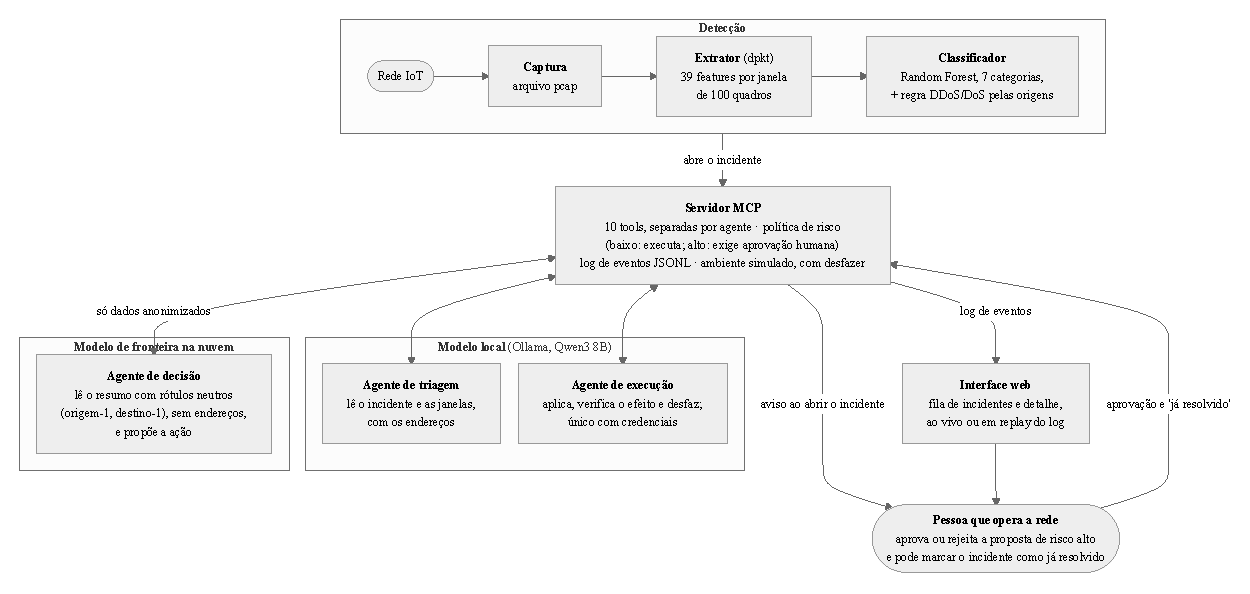
\includegraphics[width=\textwidth]{arquitetura.pdf}
	\legend{Fonte: os autores.}
\end{figure}

\begin{figure}[htb]
	\centering
	\caption{\pendente{legenda do fluxo de um incidente}}
	\label{fig:fluxo}
	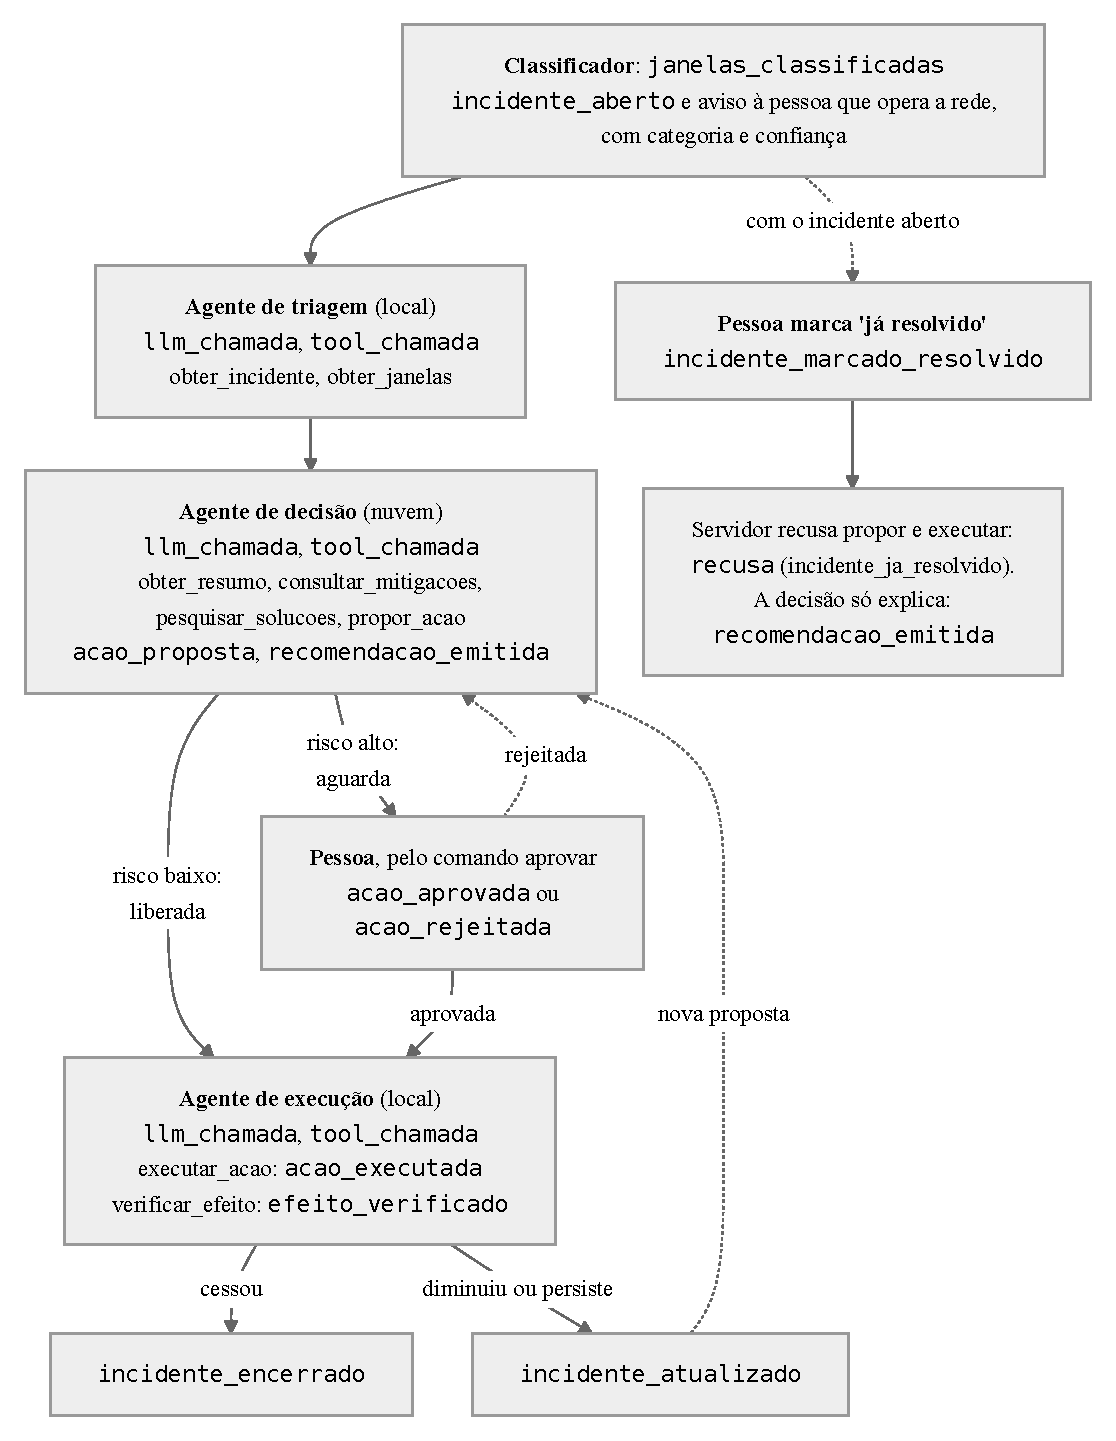
\includegraphics[width=\textwidth]{fluxo_incidente.pdf}
	\legend{Fonte: os autores.}
\end{figure}

\subsection{Avaliação da PoC e dos agentes}

\pendente{3.6, com o método do teste na casa (tarefa 93) e nos datasets externos (tarefa 95)}

% Teto: 2.500 palavras no total (4.1: 650; 4.2: 400 e uma tabela; 4.3: 650 e uma tabela;
% 4.4: 600). Fonte: 4.1 e Limitações do .docx (PR 56), tarefas 93 e 95, resultados dos agentes.
\section{Resultados e discussão}

\subsection{Classificador}

\pendente{4.1 do .docx, com as Tabelas 1 e 2 e a figura do recall com o pcap fora do treino
(PR 57)}

\begin{figure}[htb]
	\centering
	\caption{\pendente{legenda da matriz de confusão}}
	\label{fig:matriz}
	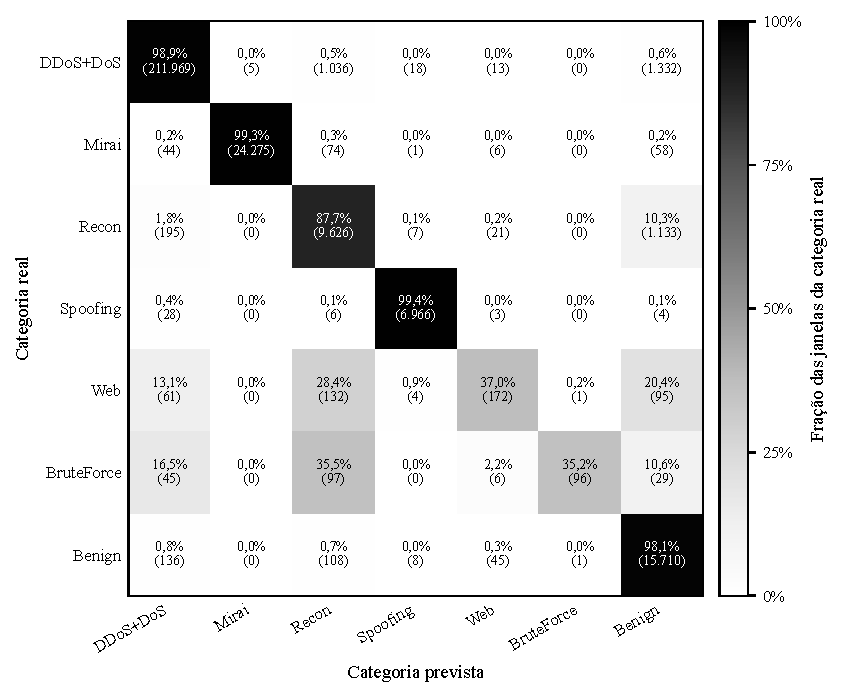
\includegraphics[width=0.8\textwidth]{matriz_confusao.pdf}
	\legend{Fonte: os autores.}
\end{figure}

\subsection{Tráfego fora do CICIoT2023}

\pendente{a casa, o IoT-23 e o CICIoMT2024 numa tabela só (tarefas 93 e 95)}

\subsection{Agentes}

\pendente{as três configurações (local, nuvem e híbrida): veredito, recomendação contra o
gabarito, custo e latência}

\subsection{Limitações}

\pendente{de 24 itens para 8 a 10}

% Teto: 400 palavras.
\section{Conclusão}

\pendente{relato do trabalho, resposta ao problema, contribuições, limitações e trabalhos
futuros}

% Declaração de uso de ferramentas de IA generativa na elaboração do trabalho (tarefa 88).
% Regra do orientador (27/10): todo uso de IA na pesquisa é explicado e apontado no artigo, por etapa,
% na voz da equipe e sem coautoria. Nem o template da FCI nem as páginas públicas da Mackenzie pedem
% formato próprio; por isso, uma seção curta antes das referências.
\section*{Declaração de uso de inteligência artificial generativa}
\label{sec:declaracao-ia}

A equipe usou ferramentas de inteligência artificial (IA) generativa na elaboração deste trabalho, nas etapas descritas abaixo. Elas não são autoras: o que produziram foi revisado pela equipe, que responde pelo conteúdo. Os modelos de linguagem que fazem parte do sistema, os agentes da seção~\ref{sec:mcp}, são objeto de estudo, e não ferramentas de elaboração, e não entram nesta declaração.

Matheus Queiroz Gregorin usou o Claude Code, assistente de programação da Anthropic, em três etapas. No código, ele gerou os scripts das figuras e o comando que as regera, e o verificador do artigo contra as regras do template, com os testes automatizados. No texto, ele redigiu, a partir do esqueleto do artigo, trechos da Introdução, das seções 2.1 e 2.2, da Metodologia e dos Resultados, as Limitações, a lista de siglas e verbetes do glossário. Na análise, ele leu o artigo de \citeonline{neto2023} para a comparação com o baseline publicado e conferiu os números do texto contra os relatórios do repositório. Tudo passou por revisão em pull request de outro integrante, pelos testes automatizados e pela integração contínua, e os números foram conferidos contra os relatórios gerados pelos scripts do projeto \cite{oliveira2026}.

\pendente{ferramentas de IA generativa de Bernardo Souza Oliveira, José Victor Roling e Pedro Henrique Cagnoni Guimarães: quais, em que etapas e como cada um conferiu o que elas produziram (tarefa 88).}


% ----------------------------------------------------------
% ELEMENTOS PÓS-TEXTUAIS
% ----------------------------------------------------------
\postextual

% Só entra na lista o que o texto cita. Não usar \nocite{*}: com o abntex2cite, ele puxa também as
% entradas de opções do abntex2-options.bib e o BibTeX falha.
\pendente{acrescentar as referências do TCC I que continuarem citadas (por exemplo, FERRAG et al., 2024).}

\bibliography{referencias}

\end{document}
